\section{Sélection d'un modèle}\label{chapter-ML-section-hyperparameters}
Le choix d'un modèle et de ses hyper-paramètres est l'objet de cette section.
Deux types de modèle sont étudiés:
\begin{itemize}
\item des arbres de décision améliorés, introduits section~\ref{chapter-ML-section-XGB}, notés XGB;
\item des réseaux de neurones profonds, introduits section~\ref{chapter-ML-section-DNN}, notés DNN.
\end{itemize}
\par
Les hyper-paramètres des XGBs sont:
\begin{itemize}
\item la profondeur maximale des arbres \MaxDepth;
\item la quantité d'échantillons minimale dans une branche \MinChildWeight;
\item le nombre d'arbres \Nestimators;
\item le gain minimal $\gamma$;
\item le taux d'apprentissage $\eta$;
\item la fonction de coût \Loss;
\item la liste des variables d'entrée.
\end{itemize}
Les hyper-paramètres des DNNs sont:
\begin{itemize}
\item le nombre de couches cachées $N_L$;
\item le nombre de neurones par couche cachée $N_N$;
\item la fonction d'activation des neurones des couches cachées;
\item la méthode d'optimisation;
\item la fonction de coût \Loss;
\item le mode d'initiation des poids;
\item la liste des variables d'entrée.
\end{itemize}
\par
Il est difficile de définir un seul score quantifiant la qualité d'un modèle.
Plusieurs métriques sont considérées afin d'évaluer les modèles:
\begin{itemize}
\item les valeurs de
\LossMSE,
\LossMAE,
\LossMAPE;
\item la largeur du premier quantile de la distribution des réponses des modèles,
ou \og largeur à $1\sigma$ \fg,
notée \OneSigmaWidth,
où la réponse $r$ est définie comme
\begin{equation}
r = \frac{\ypred}{\ytrue} = \frac{F(\vec{x})}{m_{\higgsML}}
\mend
\end{equation}
\end{itemize}
Pour toutes ces métriques, l'objectif est la plus petite valeur possible.
De plus, quatre domaines de masse sont définis:
\begin{itemize}
\item basse masse : $m_{\higgsML} < \SI{150}{\GeV}$, incluant en particulier les bosons \Zboson\ et \higgs;
\item masse moyenne : $\SI{150}{\GeV} \geq m_{\higgsML} < \SI{500}{\GeV}$;
\item haute masse : $m_{\higgsML} \geq \SI{500}{\GeV}$;
\item toute masse : aucune restriction sur $m_{\higgsML}$.
\end{itemize}
Ils permettent de comparer les performances des modèles sur certaines gammes de masse uniquement.
Sauf contre-indication, toute la gamme de masse est considérée.
\subsection{Variables d'entrée}
Les différentes variables d'entrée considérées sont listées dans la section~\ref{chapter-ML-section-evt_gen-inputs}.
La plupart de celles-ci sont généralement déjà exploitées dans les analyses en cours.
Ce n'est toutefois pas garanti, en particulier pour les variables relatives à l'activité hadronique additionnelle.
L'utilisation de variables supplémentaires demande,
en plus de la mise en place de leur obtention,
de reprendre potentiellement de longues étapes de calculs.
Se restreindre à un sous-ensemble des variables d'entrée,
si cela ne dégrade pas la qualité des modèles,
pourrait donc faciliter l'intégration de nos modèles.
\par
Les sous-ensembles des variables d'entrée sont définis par les restrictions suivantes:
\begin{itemize}
\item sans \Npu: la variable \Npu\ n'est pas utilisée;
\item sans \Nnu: la variable \Nnu\ n'est pas utilisée;
\item sans AHA: les variables d'activité hadronique additionnelle ne sont pas utilisées;
\item sans jets: les variables relatives aux jets (dont AHA) ne sont pas utilisées;
\item sans \mT: les masses transverses ne sont pas utilisées;
\item sans METcov: la matrice de covariance de \MET\ n'est pas utilisée.
\end{itemize}
L'application de plusieurs de ces restrictions est également testée.
\par
Les performances modèles entraînés avec les différents ensembles de variables d'entrée sont données
figure~\ref{fig-XGB_inputs} pour les XGBs
et
figure~\ref{fig-DNN_inputs}
pour les DNNs.
Les modèles concernés par plusieurs restrictions sont comptés de manière pondérée dans chaque groupe correspondant à une restriction unique.
Par exemple, un modèle soumis à la restriction \og sans \Npu\ \fg{} et \og sans \Nnu\ \fg{} aura un poids de $\frac{1}{2}$ dans chacun de ces deux groupes.
Une pondération par la quantité de modèles dans chaque groupe est de plus appliquée pour supprimer le biais lié à la quantité accrue de modèles dans le groupe sans restrictions.
Les histogrammes ainsi créés sont superposés.
Il est alors possible de voir les contributions de chacune des restrictions aux valeurs obtenues sur la métrique d'évaluation illustrée.
\begin{figure}[h]
\centering

\subcaptionbox{\label{subfig-XGB_inputs-mape}}[.45\textwidth]
{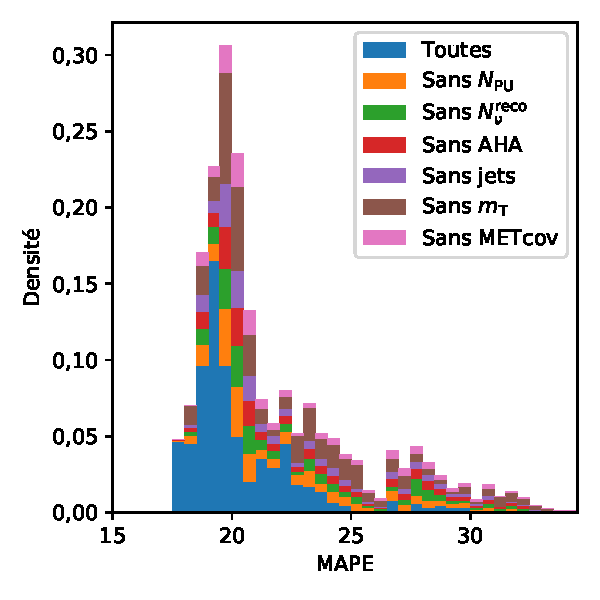
\includegraphics[width=.45\textwidth]{\PhDthesisdir/plots_and_images/my_plots/ML/from_ML_plots/global_comparisons/XGB_inputs_all-full_mape.pdf}\vspace{-\baselineskip}}
\hfill
\subcaptionbox{\label{subfig-XGB_inputs-1sigw}}[.45\textwidth]
{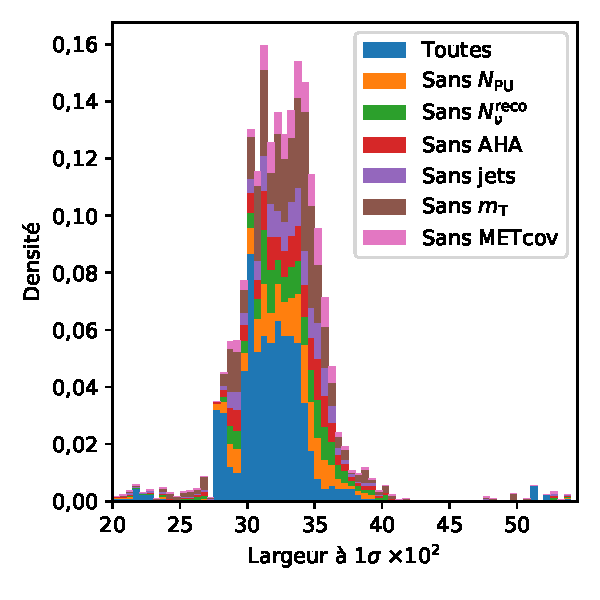
\includegraphics[width=.45\textwidth]{\PhDthesisdir/plots_and_images/my_plots/ML/from_ML_plots/global_comparisons/XGB_inputs_all-full_1sig_width.pdf}\vspace{-\baselineskip}}

\caption{Comparaison des performances des XGBs selon les variables d'entrée.}
\label{fig-XGB_inputs}
\end{figure}
\begin{figure}[h]
\centering

\subcaptionbox{\label{subfig-DNN_inputs-mape}}[.45\textwidth]
{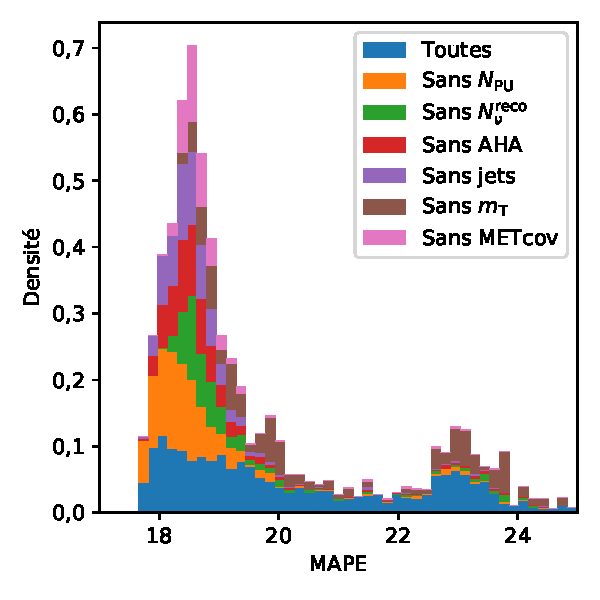
\includegraphics[width=.45\textwidth]{\PhDthesisdir/plots_and_images/my_plots/ML/from_ML_plots/global_comparisons/DNN_inputs_all-full_mape.pdf}\vspace{-\baselineskip}}
\hfill
\subcaptionbox{\label{subfig-DNN_inputs-1sigw}}[.45\textwidth]
{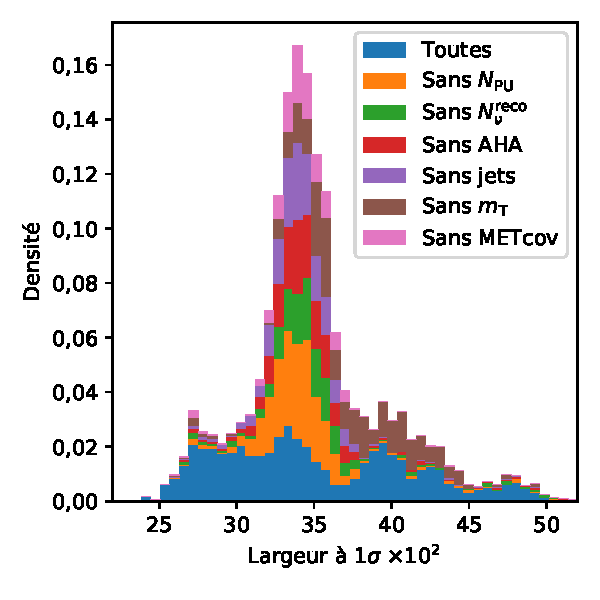
\includegraphics[width=.45\textwidth]{\PhDthesisdir/plots_and_images/my_plots/ML/from_ML_plots/global_comparisons/DNN_inputs_all-full_1sig_width.pdf}\vspace{-\baselineskip}}

\caption{Comparaison des performances des DNNs selon les variables d'entrée.}
\label{fig-DNN_inputs}
\end{figure}
\par
Dans le cas des XGBs,
l'évaluation des modèles par \LossMAPE, en figure~\ref{subfig-XGB_inputs-mape},
montre que les modèles utilisant toutes les variables d'entrée permettent d'obtenir plus facilement
une faible valeur de cette métrique.
Le coeur de la distribution,
aux alentours de $\LossMAPE=\todo{?}$,
est en effet plutôt constitué
de modèles utilisant
toutes les entrées
dans sa partie gauche (\LossMAPE\ faible)
et
de modèles utilisant
un sous-ensemble d'entrées
dans sa partie droite (\LossMAPE\ haute).
De plus, les basses valeurs de \LossMAPE, en-dessous de \todo{?},
sont presque exclusivement obtenues avec des modèles utilisant toutes les entrées.
À l'inverse, la queue à hautes valeurs de la distribution obtenue est largement dominée par les contributions des modèles avec un sous-ensemble d'entrées.
\par
La largeur \OneSigmaWidth, en figure~\ref{subfig-XGB_inputs-1sigw},
montre des extremums
à \todo{?} et \todo{?}
pour l'ensemble des modèles,
mais
à \todo{?} et \todo{?}
pour les modèles utilisant toutes les entrées.
Quelques modèles sans \mT\ présentent
une valeur de \OneSigmaWidth\
inférieure à \todo{?},
mais ils sont associés à des valeurs de \LossMAPE\
plus élevées que ceux utilisant toutes les entrées.
\par
Dans le cas des DNNs,
la métrique \LossMAPE, en figure~\ref{subfig-DNN_inputs-mape},
ne montre pas d'avantage net d'un type de modèle sur un autre.
En revanche,
la largeur \OneSigmaWidth, en figure~\ref{subfig-DNN_inputs-1sigw},
montre que les modèles utilisant toutes les entrées peuvent se répartir en trois groupes,
aux alentour des valeurs
\todo{?}, \todo{?} et \todo{?}.
À \todo{?3e} apparaît également un groupe de modèles entraînés sans \mT.
À \todo{?2e} se trouvent la majorité des modèles entraînés avec une restriction des entrées.
Les modèles de ces groupes ont potentiellement minimisé l'utilisation de certaines variables.
Les modèles d'intérêt sont ceux du groupe se situant à \OneSigmaWidth\ d'environ \todo{?1er}.
Il s'agit presque exclusivement de modèles utilisant toutes les variables d'entrée.
\par
L'utilisation de toutes les variables listées dans la section~\ref{chapter-ML-section-evt_gen-inputs}
est ainsi corrélée avec de meilleures performances
selon les métriques
\LossMAPE\
et \OneSigmaWidth.
Par la suite, seuls les modèles utilisant toutes les variables, au nombre de 27, sont considérés.

\subsection{Type de modèle}
Les distributions des métriques des deux types de modèle sont données figure~\ref{fig-DNN_vs_XGB}.
Si les XGBs sont compétitifs selon \OneSigmaWidth, les DNNs proposent de bien meilleures performances sur \LossMSE, \LossMAE\ et surtout \LossMAPE.
La sélection d'un modèle est donc faite parmi les DNNs.
\begin{figure}[h]
\centering

\subcaptionbox{}[.45\textwidth]
{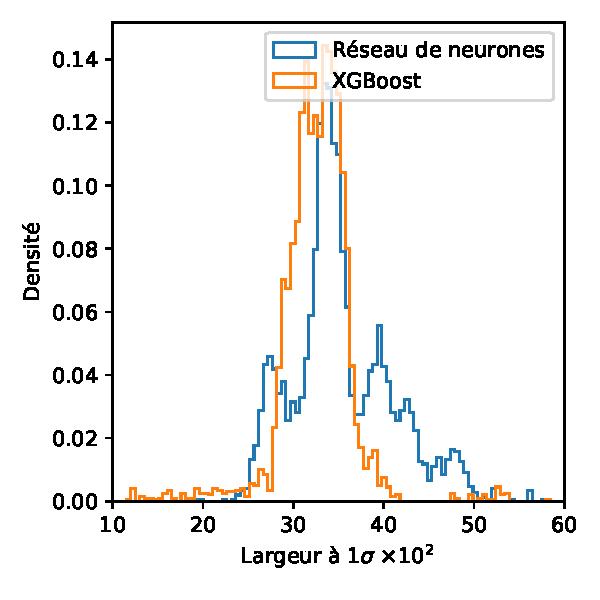
\includegraphics[width=.45\textwidth]{\PhDthesisdir/plots_and_images/my_plots/ML/from_ML_plots/global_comparisons/DNN_vs_XGB-full_1sig_width.pdf}\vspace{-\baselineskip}}
\hfill
\subcaptionbox{}[.45\textwidth]
{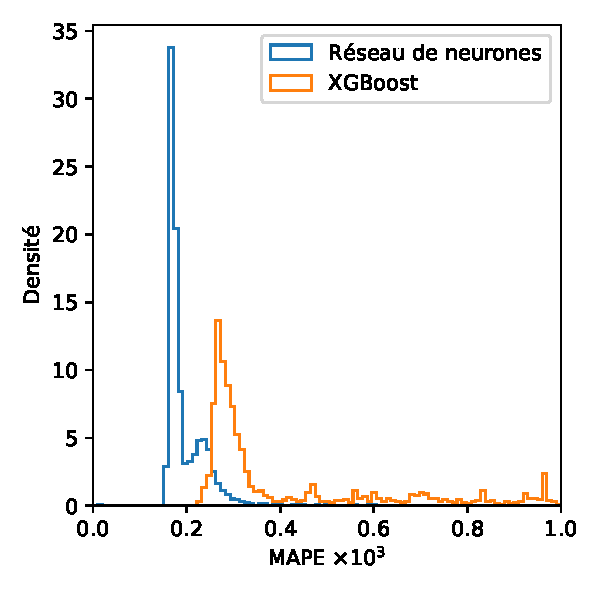
\includegraphics[width=.45\textwidth]{\PhDthesisdir/plots_and_images/my_plots/ML/from_ML_plots/global_comparisons/DNN_vs_XGB-full_mape.pdf}\vspace{-\baselineskip}}

\vspace{\baselineskip}

\subcaptionbox{}[.45\textwidth]
{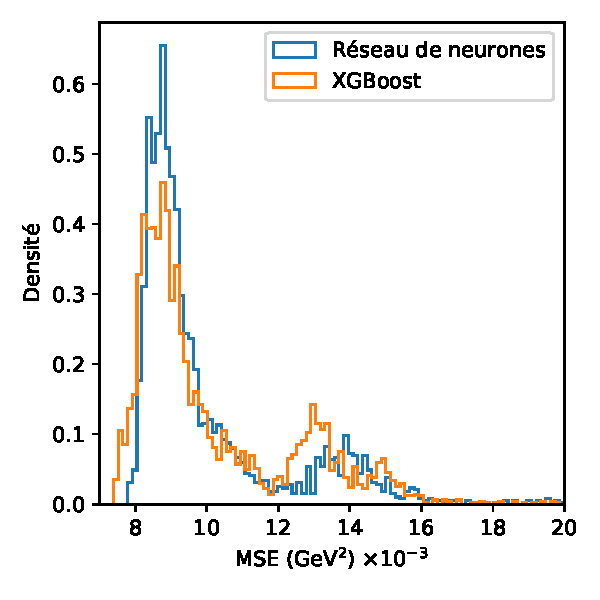
\includegraphics[width=.45\textwidth]{\PhDthesisdir/plots_and_images/my_plots/ML/from_ML_plots/global_comparisons/DNN_vs_XGB-full_mse.pdf}\vspace{-\baselineskip}}
\hfill
\subcaptionbox{}[.45\textwidth]
{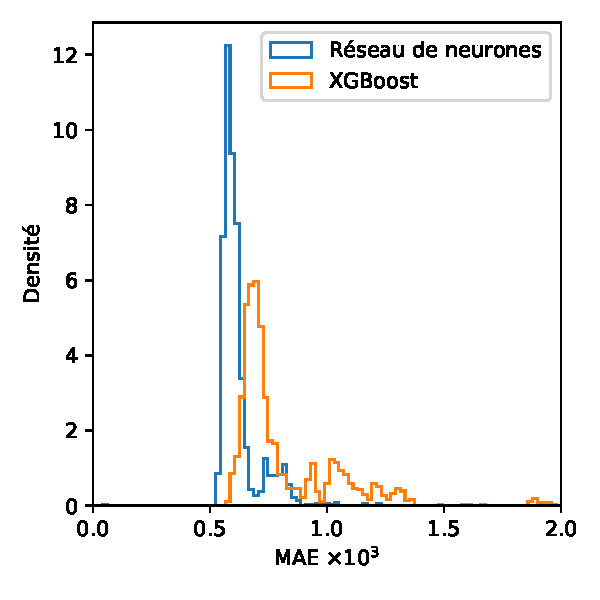
\includegraphics[width=.45\textwidth]{\PhDthesisdir/plots_and_images/my_plots/ML/from_ML_plots/global_comparisons/DNN_vs_XGB-full_mae.pdf}\vspace{-\baselineskip}}

\caption{Comparaisons des XGBs et des DNNs.}
\label{fig-DNN_vs_XGB}
\end{figure}
\newpage
\subsection{Fonction de coût}
Le choix de la fonction de coût \Loss\ ne peut se faire sur la base des métriques correspondant elles-mêmes.
En effet, comme cela se voit sur la figure~\ref{fig-loss_mse_mape_themselves},
les réseaux entraînés de manière à minimiser une fonction de coût sont meilleurs selon cette métrique.
\begin{figure}[h]
\centering

\subcaptionbox{}[.45\textwidth]
{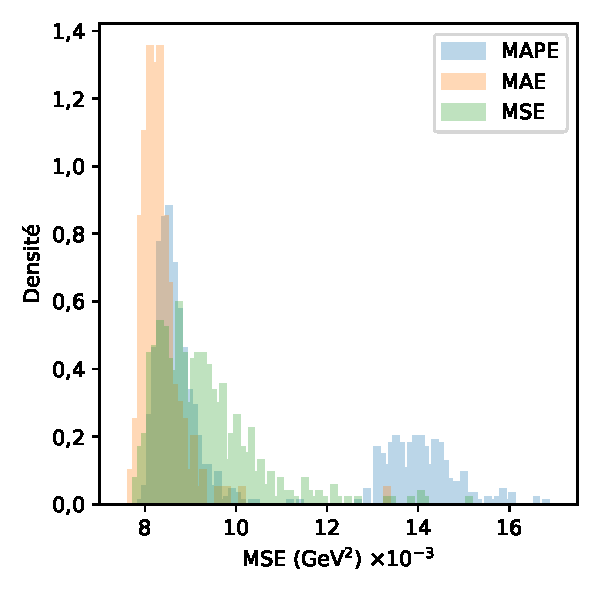
\includegraphics[width=.45\textwidth]{\PhDthesisdir/plots_and_images/my_plots/ML/from_ML_plots/global_comparisons/DNN_loss-full_mse.pdf}\vspace{-\baselineskip}}
\hfill
\subcaptionbox{}[.45\textwidth]
{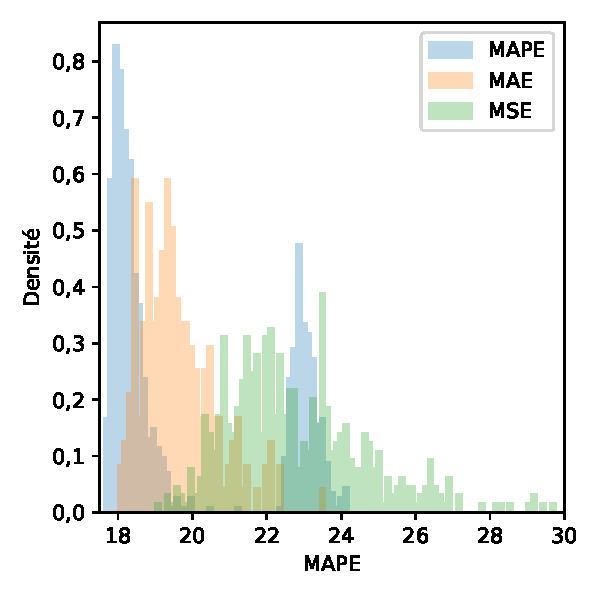
\includegraphics[width=.45\textwidth]{\PhDthesisdir/plots_and_images/my_plots/ML/from_ML_plots/global_comparisons/DNN_loss-full_mape.pdf}\vspace{-\baselineskip}}

\caption{Comparaisons des fonctions de coût \LossMSE\ et \LossMAPE\ d'après leurs propres valeurs.}
\label{fig-loss_mse_mape_themselves}
\end{figure}
\par
Cependant, l'écart entre les modèles minimisant \LossMSE\ ou bien \LossMAPE\
est moindre lorsqu'ils sont évalués par \LossMSE\ que par \LossMAPE,
ce qui laisse à penser que l'utilisation de \LossMAPE\ donne de meilleurs modèles.
Ceci est confirmé par la figure~\ref{fig-loss_mse_mape_by_mae_and_low_1sigma} où ces deux catégories de modèles sont évaluées par \LossMAE\ et par \OneSigmaWidth\ à basse masse.
La fonction de coût retenue est donc \LossMAPE.
\begin{figure}[h]
\centering

\subcaptionbox{}[.45\textwidth]
{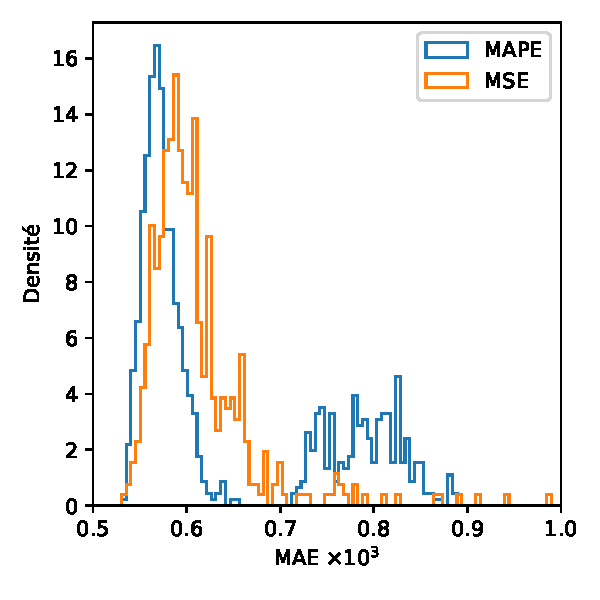
\includegraphics[width=.45\textwidth]{\PhDthesisdir/plots_and_images/my_plots/ML/from_ML_plots/global_comparisons/DNN_loss-full_mae.pdf}\vspace{-\baselineskip}}
\hfill
\subcaptionbox{}[.45\textwidth]
{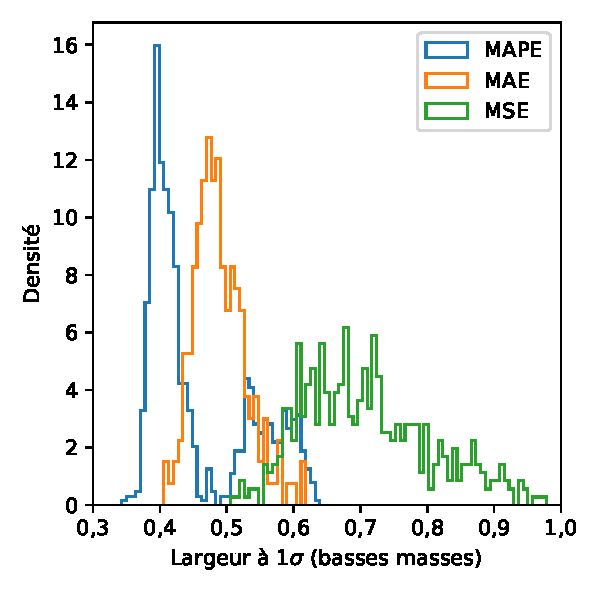
\includegraphics[width=.45\textwidth]{\PhDthesisdir/plots_and_images/my_plots/ML/from_ML_plots/global_comparisons/DNN_loss-low_1sig_width.pdf}\vspace{-\baselineskip}}

\caption{Comparaisons des fonctions de coût \LossMSE\ et \LossMAPE\ d'après d'autres métriques.}
\label{fig-loss_mse_mape_by_mae_and_low_1sigma}
\end{figure}
\newpage
\subsection{Algorithme d'optimisation et initiation des paramètres}
Trois algorithmes d'optimisation ont été considérés, SGD, Adadelta et Adam.

\todo{QGD complètement dans les choux}

Il apparaît sur la figure~\ref{fig-optimizer} qu'Adam propose de meilleurs modèles qu'Adadelta.
L'initiation des paramètres des neurones n'a en revanche que peu d'influence sur \LossMAPE, comme cela se voit figure~\ref{fig-w_init_mode}.
\begin{figure}[h]
\centering

\subcaptionbox{}[.45\textwidth]
{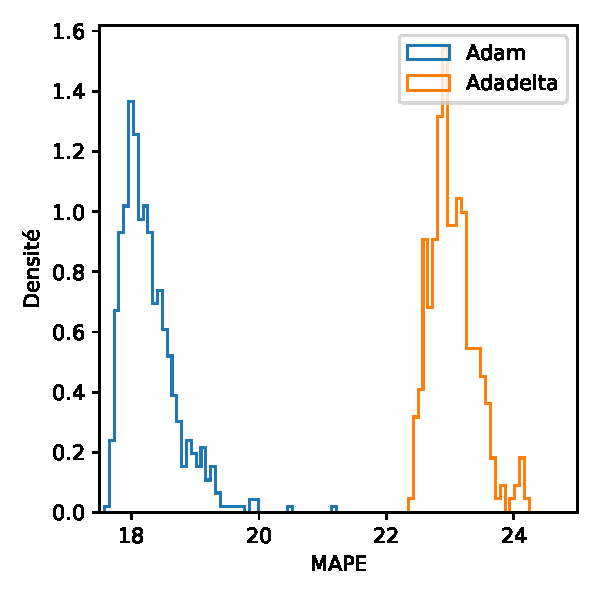
\includegraphics[width=.45\textwidth]{\PhDthesisdir/plots_and_images/my_plots/ML/from_ML_plots/global_comparisons/DNN_optimizer-full_mape.pdf}\vspace{-\baselineskip}}
\hfill
\subcaptionbox{}[.45\textwidth]
{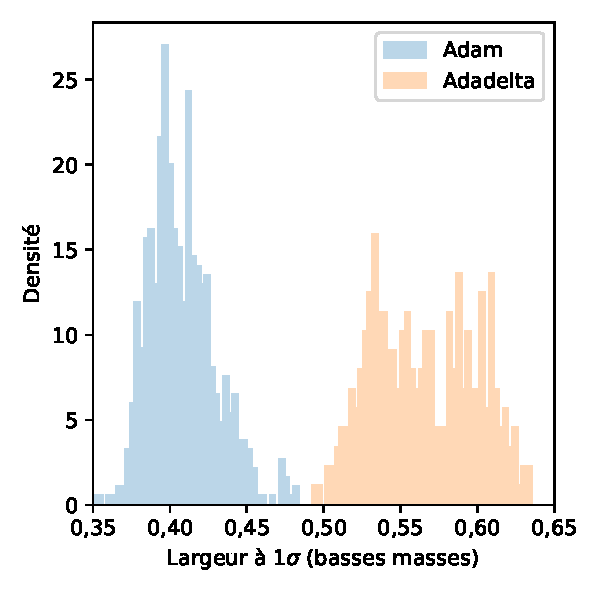
\includegraphics[width=.45\textwidth]{\PhDthesisdir/plots_and_images/my_plots/ML/from_ML_plots/global_comparisons/DNN_optimizer-low_1sig_width.pdf}\vspace{-\baselineskip}}
\caption{Comparaisons des algorithmes d'optimisation.}
\label{fig-optimizer}
\end{figure}
\begin{figure}[h]
\centering
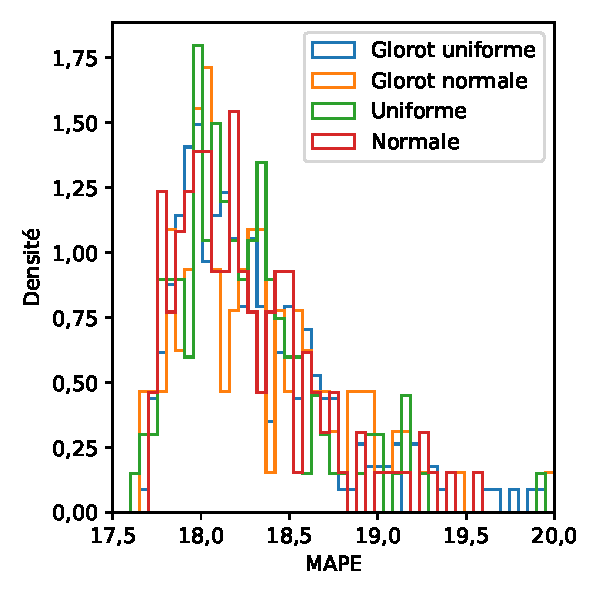
\includegraphics[width=.45\textwidth]{\PhDthesisdir/plots_and_images/my_plots/ML/from_ML_plots/global_comparisons/DNN_w_init_mode-full_mape.pdf}
\caption{Comparaisons des initiations des paramètres.}
\label{fig-w_init_mode}
\end{figure}
\subsection{Structure}
which structure ?

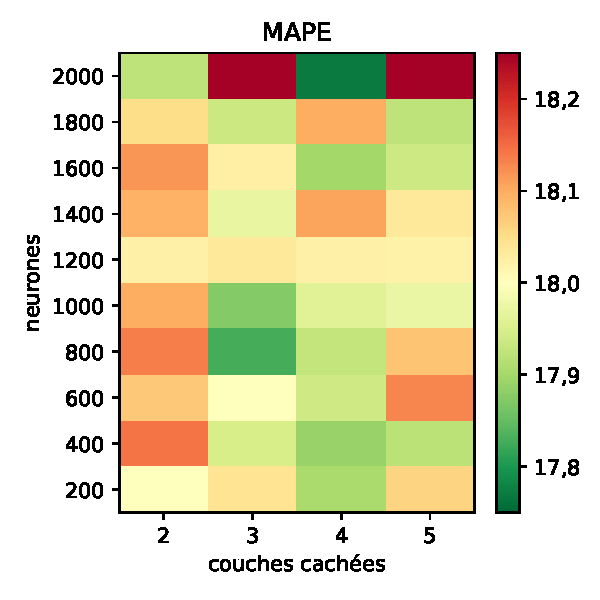
\includegraphics[width=.45\textwidth]{\PhDthesisdir/plots_and_images/my_plots/ML/from_ML_plots/global_comparisons/DNN_structures_reduced-full_mape.pdf}
%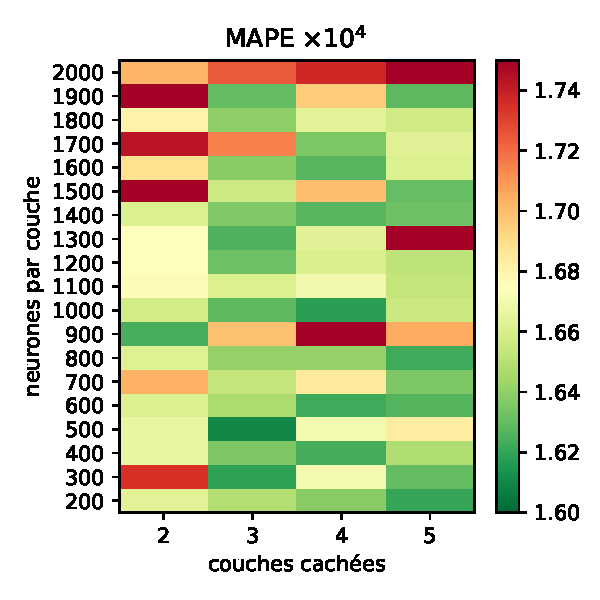
\includegraphics[width=.45\textwidth]{\PhDthesisdir/plots_and_images/my_plots/ML/from_ML_plots/global_comparisons/DNN_structures_all-full_mape.pdf}

several possibilities, but the loss mass region contains the Z boson and is important

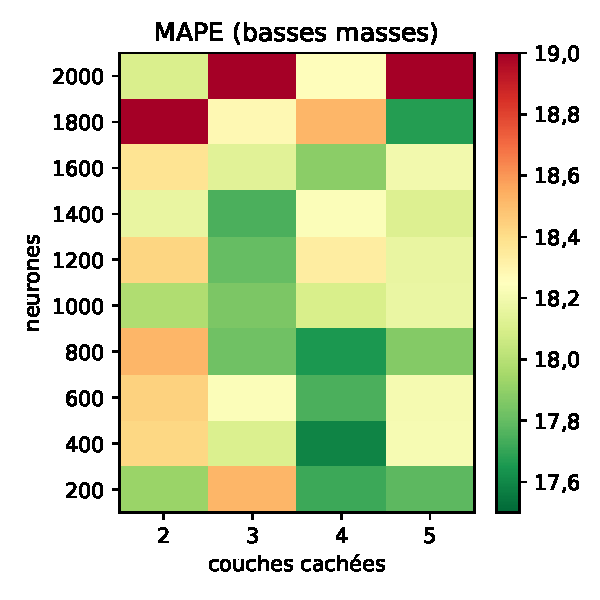
\includegraphics[width=.45\textwidth]{\PhDthesisdir/plots_and_images/my_plots/ML/from_ML_plots/global_comparisons/DNN_structures_reduced-low_mape.pdf}
%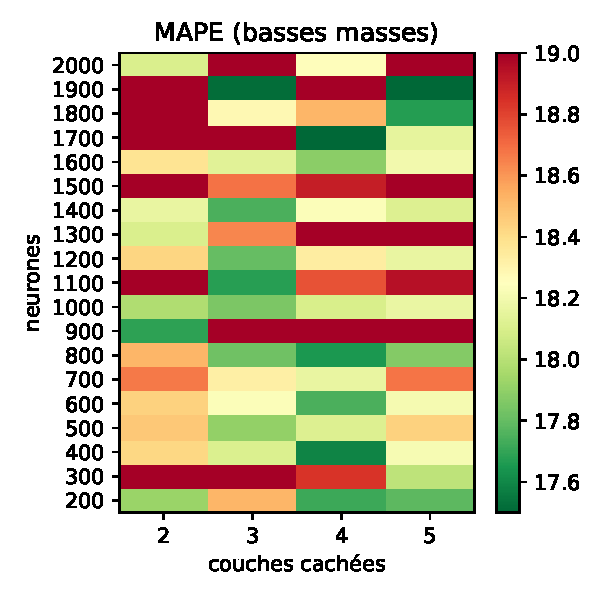
\includegraphics[width=.45\textwidth]{\PhDthesisdir/plots_and_images/my_plots/ML/from_ML_plots/global_comparisons/DNN_structures_all-low_mape.pdf}

2x900 and 5x600 seem to be the best options, check the low mass resolution

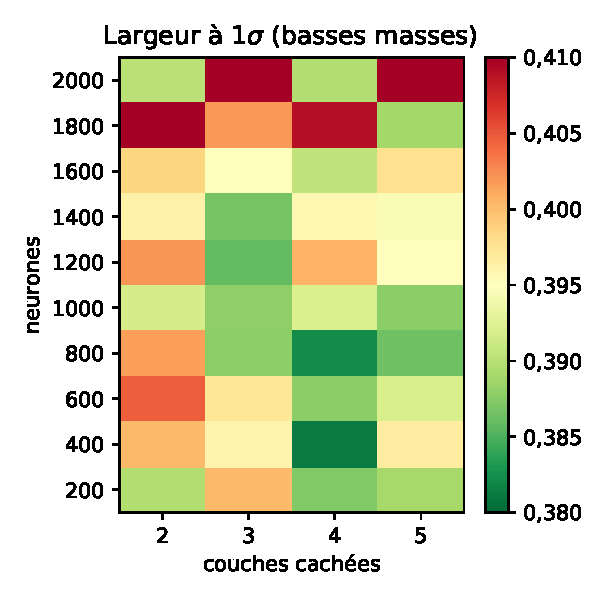
\includegraphics[width=.45\textwidth]{\PhDthesisdir/plots_and_images/my_plots/ML/from_ML_plots/global_comparisons/DNN_structures_reduced-low_1sig_width.pdf}
%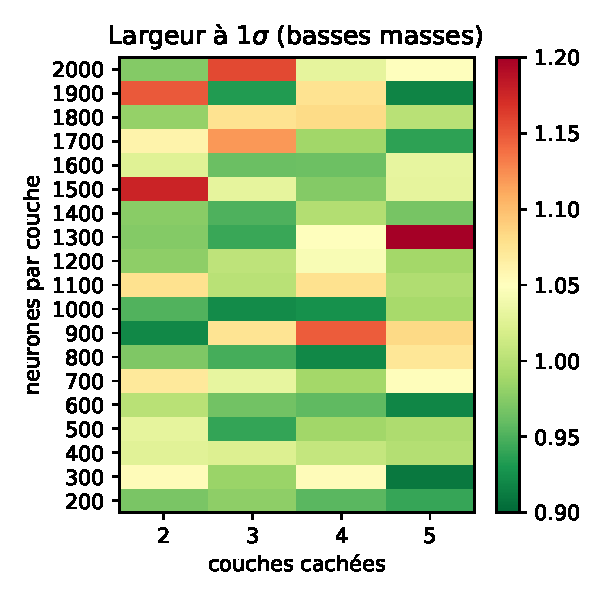
\includegraphics[width=.45\textwidth]{\PhDthesisdir/plots_and_images/my_plots/ML/from_ML_plots/global_comparisons/DNN_structures_all-low_1sig_width.pdf}

5x600 seems good, check the low mass \textbf{calibrated} resolution

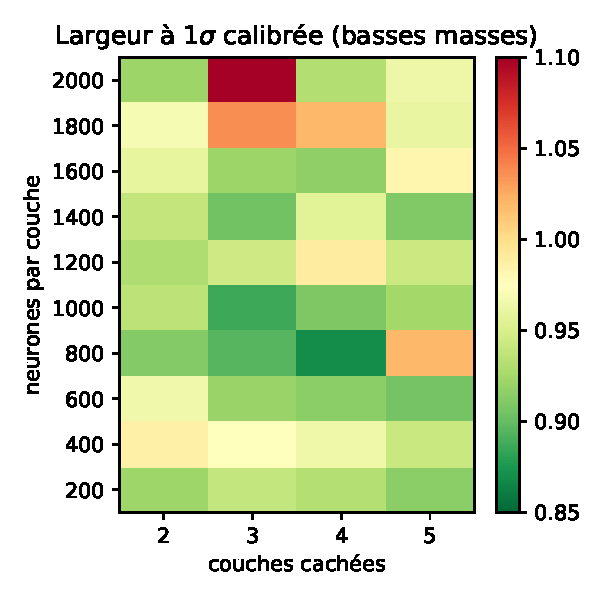
\includegraphics[width=.45\textwidth]{\PhDthesisdir/plots_and_images/my_plots/ML/from_ML_plots/global_comparisons/DNN_structures_reduced-low_1sig_calibr_width.pdf}
%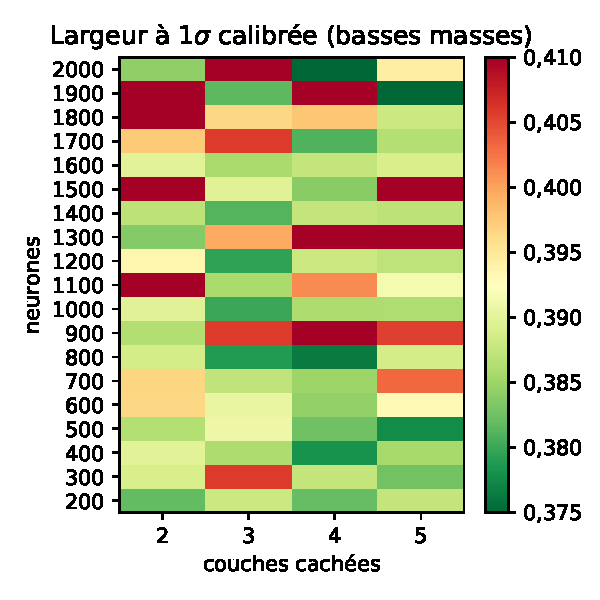
\includegraphics[width=.45\textwidth]{\PhDthesisdir/plots_and_images/my_plots/ML/from_ML_plots/global_comparisons/DNN_structures_all-low_1sig_calibr_width.pdf}

and in the medium mass region we have

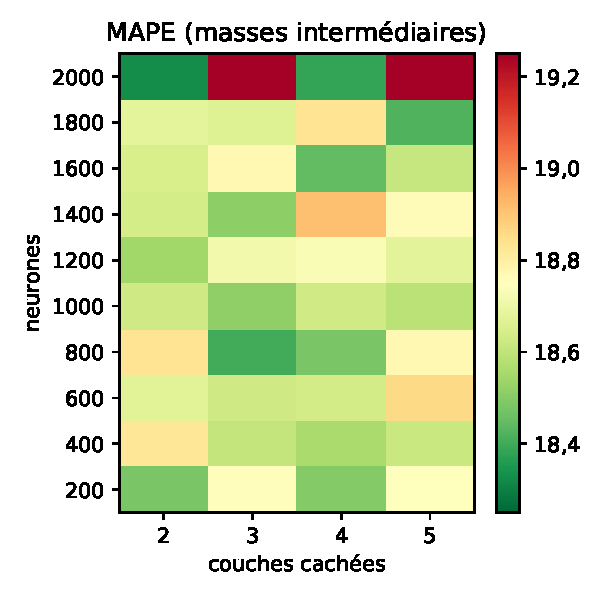
\includegraphics[width=.45\textwidth]{\PhDthesisdir/plots_and_images/my_plots/ML/from_ML_plots/global_comparisons/DNN_structures_reduced-medium_mape.pdf}
%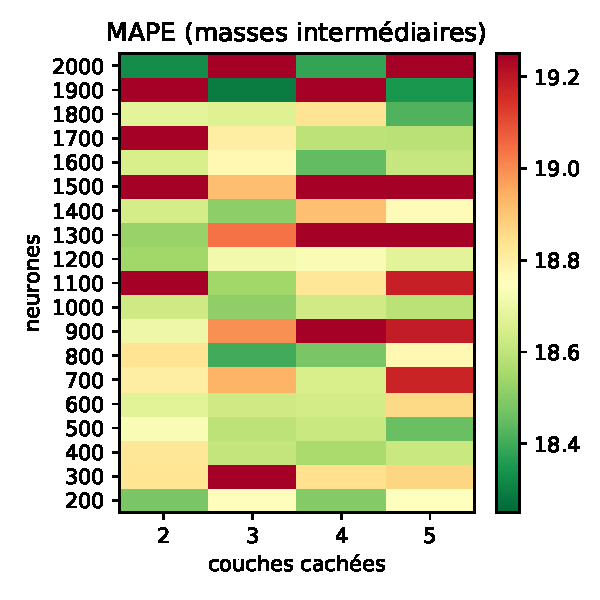
\includegraphics[width=.45\textwidth]{\PhDthesisdir/plots_and_images/my_plots/ML/from_ML_plots/global_comparisons/DNN_structures_all-medium_mape.pdf}

3x1000 is the best compromise we found

\subsection{Fonction d'activation}

activation = softplus

